\noindent
\textbf{Thermodynamics:
\ifthenelse{\equal{\solutions}{true}}{Examples}{Homework} for chapter 1.}\\

\begin{enumerate}
\item When 0.12 g of solid iodine was vaporized at 1670 K, the resulting gas displaced 20.2 cm$^3$ of dry air at 298 K and 99.9 kPa pressure. How many iodine molecules were dissociated (i.e. as atomic iodine) in the gas? The gas phase equilibrium reaction is:

$$\textnormal{I}_2(g) \rightleftharpoons 2\textnormal{I}(g)$$

Assume that the gas mixture (of I$_2$ and I) behave according to the ideal gas law.

\ifthenelse{\equal{\solutions}{true}}{% Problem 1/1 solution
\noindent
\underline{Solution:}\\

% FIX This: is it clear that we should use 298 K and not 1680 K

The amount of I$_2$ before any dissociation takes place is:

$$n = \frac{m}{M_{\textnormal{I}_2}} = \frac{0.12\textnormal{ g}}{254\textnormal{ g mol}^{-1}} = 4.7\times 10^{-4}\textnormal{ mol}$$

After the equilibrium has been reached, the amount of I$_2$ is $(1 - \alpha)n$ and the amount of I is $2\alpha n$. Here the degree of dissociation is denoted by $\alpha$. The ideal gas law is:

$$PV = nRT \Rightarrow n = \frac{PV}{RT} \Rightarrow n = (1 - \alpha)n + 2\alpha n = \frac{PV}{RT}$$

$$\Rightarrow \alpha = \frac{PV}{nRT} - 1$$

$$ = \frac{PVM_{\textnormal{I}_2}}{mRT} - 1 = \frac{(99.9\textnormal{ kN m}^{-2})\times(20.2\times 10^{-6}\textnormal{m}^3)\times(254\textnormal{ g mol}^{-1})}{(0.12\textnormal{ g})\times(8.31\textnormal{ J K}^{-1}\textnormal{ mol}^{-1})\times(298\textnormal{ K})} = 0.72$$

The amount of I is $2\alpha n = 2\times 0.72\times\left(4.7\times 10^{-4}\textnormal{ mol}\right) = 6.8\times 10^{-4}\textnormal{ mol}$.
\hrule\vspace{0.5cm}
}{}

\item What is the molar volume of $n$-hexane at 660 K and 91 bar according to (a) the ideal gas law and (b) the van der Waals equation? For $n$-hexane, $T_c$ = 507.7 K and $P_c$ = 30.3 bar. If you obtain an equation that you cannot solve analytically, attempt to solve it
numerically.

\ifthenelse{\equal{\solutions}{true}}{% Problem 2/1 solution
\noindent
\underline{Solution:}\\
\begin{enumerate}
\item
\begin{itemize}
\item $\frac{d(e^{ikx})}{dx} = ike^{ikx} = \textnormal{``constant} \times \textnormal{original function''}$. Thus this is an eigenfunction of the given operator.
\item $\frac{d^2(e^{ikx}}{dx^2} = \frac{d}{dx}(ike^{ikx}) = -k^2e^{ikx} = \textnormal{``constant} \times \textnormal{original function''}$. Thus this is an eigenfunction of the given operator.
\item $\frac{d(k)}{dx} = \frac{d^2(k)}{dx^2} = 0$. This could be considered as en eigenfunction with zero eigenvalue.
\item $\frac{d(e^{ax^2})}{dx} = 2axe^{ax^2} \ne$ ``constant $\times$ original function'', thus not an eigenfunction.
\item $\frac{d^2(e^{ax^2})}{dx^2} = \frac{d(2axe^{ax^2})}{dx} = 2a(2ax^2 + 1)e^{ax^2} \ne$ ``constant $\times$ original function'', thus not an eigenfunction.
\item $\frac{d(\cos(x))}{dx} = -\sin(x)$. Not an eigenfunction.
\item $\frac{d^2(\cos(x))}{dx^2} = \frac{d(-\sin(x))}{dx} = -\cos(x)$. This is an eigenfunction (with eigenvalue -1).
\end{itemize}
\item $f(x, y, z) = \cos(ax)\cos(by)\cos(cz)$. The partial derivatives are:
$$\frac{\partial f(x,y,z)}{\partial x} = -a\sin(ax)\cos(by)\cos(cz)$$
$$\frac{\partial f(x,y,z)}{\partial y} = -b\cos(ax)\sin(by)\cos(cz)$$
$$\frac{\partial f(x,y,z)}{\partial z} = -c\cos(ax)\cos(by)\sin(cz)$$
and
$$\frac{\partial^2 f(x,y,z)}{\partial x^2} = -a^2\cos(ax)\cos(by)\cos(cz)$$
$$\frac{\partial^2 f(x,y,z)}{\partial y^2} = -b^2\cos(ax)\cos(by)\cos(cz)$$
$$\frac{\partial^2 f(x,y,z)}{\partial z^2} = -c^2\cos(ax)\cos(by)\cos(cz)$$
Therefore $\Delta f(x,y,z) = -(a^2 + b^2 + c^2)f(x,y,z)$ = ``constant $\times$ original function'' and this is an eigenfunction with
the corresponding eigenvalue $-(a^2 + b^2 + c^2)$.
\item The standard deviation can be calculated as:
\begin{eqnarray}
\nonumber
& & \psi_0(r) = \frac{1}{\sqrt{\pi a_0^3}} e^{-r/a_0}\\
\nonumber
& & \left<\hat{r}^2\right> = \frac{1}{\pi a_0^3}\int\limits_{0}^{\infty}e^{-2r/a_0}r^2\underbrace{4\pi r^2 dr}_{d\tau} = \frac{4}{a_0^3}\times\frac{3a_0^5}{4} = 3a_0^2\\
\nonumber
& & \left<\hat{r}\right> = \frac{1}{\pi a_0^3}\int\limits_{0}^{\infty}e^{-2r/a_0}r\underbrace{4\pi r^2 dr}_{d\tau} = \frac{3a_0}{2}\\
\nonumber
& & \left<\hat{r}\right>^2 = \frac{9a_0^2}{4}\\
\nonumber
& & \left<\hat{r}^2\right> - \left<\hat{r}\right>^2 = 3a_0^2 - \frac{9a_0^2}{4} = \frac{4a_0^2}{4}\\
\nonumber
& & \sqrt{\left<\hat{r}^2\right> - \left<\hat{r}\right>^2} = \frac{\sqrt{3}}{2}a_0\approx 0.87a_0
\end{eqnarray}
\item The potential energy expectation can be calculated as:
\begin{eqnarray}
\nonumber
& & \psi_0(r) = \frac{1}{\sqrt{\pi a_0^3}}e^{-r/a_0}\textnormal{ and }V(r) = -\frac{e^2}{4\pi\epsilon_0r}\\
\nonumber
& & \left<\hat{V}\right> = -\frac{e^2}{4\pi^2\epsilon_0a_0^3}\int\limits_{r=0}^{\infty}e^{-2r/a_0}\frac{1}{r}\underbrace{4\pi r^2dr}_{d\tau} = -\frac{e^2}{\pi\epsilon_0a_0^3}\int\limits_{r=0}^{\infty}e^{-2r/a_0}rdr\\
\nonumber
& & = -\frac{e^2}{\pi\epsilon_0a_0^3}\times\frac{a_0^2}{4} = -\frac{e^2}{4\pi\epsilon_0a_0}\approx -27.2\textnormal{ eV}
\end{eqnarray}
\end{enumerate}

\hrule\vspace{0.5cm}
}{}

\item Ten grams of N$_2$ is mixed with 5 g of O$_2$ and held at 25 $^\circ$C and 0.750 bar. (a) What are the partial pressures of N$_2$ and O$_2$? (b) What is the volume of the ideal mixture?

\ifthenelse{\equal{\solutions}{true}}{% Problem 3/1 solution
\noindent
\underline{Solution:}\\
\begin{enumerate}
\item 
\begin{eqnarray}
\nonumber
& & \psi(x) = \left(\frac{\pi}{\alpha}\right)^{-1/4}e^{-\alpha x^2/2}\\
\nonumber
& & \hat{p}_x = -i\hbar\frac{d}{dx}\textnormal{ and }\left[\hat{x},\hat{p}_x\right]\psi(x) = \left(\hat{x}\hat{p}_x - \hat{p}_x\hat{x}\right)\psi(x)
\end{eqnarray}

To obtain the commutator, we need to operate with $\hat{x}$ and $\hat{p}_x$:
\begin{eqnarray}
\nonumber
& & \left(\hat{x}\hat{p}_x\right)\psi(x) = -i\hbar\left(\frac{\pi}{\alpha}\right)^{-1/4}x\frac{d}{dx}e^{-\alpha x^2/2} = i\hbar\alpha\left(\frac{\pi}{\alpha}\right)^{-1/4}x^2e^{-\alpha x^2/2}\\
\nonumber
& & \left(\hat{p}_x\hat{x}\right)\psi(x) = -i\hbar\left(\frac{\pi}{\alpha}\right)^{-1/4}\frac{d}{dx}\left(xe^{-\alpha x^2/2}\right)\\
\nonumber
& & = i\hbar\alpha\left(\frac{\pi}{\alpha}\right)^{-1/4}x^2e^{-\alpha x^2/2} - i\hbar\left(\frac{\pi}{\alpha}\right)^{-1/4}e^{-\alpha x^2/2}
\end{eqnarray}

When these are subtracted, we get:

\begin{eqnarray}
\nonumber
& & \left(\hat{x}\hat{p}_x\right)\psi(x) - \left(\hat{p}_x\hat{x}\right)\psi(x) = i\hbar\left(\frac{\pi}{\alpha}\right)^{-1/4}e^{-\alpha x^2/2}
\end{eqnarray}

When the wavefunction $\psi(x)$ is removed, we have:
$$\left[\hat{x},\hat{p}_x\right] = i\hbar$$

Because the commutator between these operators is non-zero, it means that they are complementary.

\item The commutator for the given function is:
\begin{eqnarray}
\nonumber
& & \left[\hat{x},\hat{I}\right]\psi(x) = \left(\hat{x}^2\hat{I} - \hat{I}\hat{x}^2\right)\left(\frac{\pi}{\alpha}\right)^{-1/4}e^{-\alpha x^2/2}\\
\nonumber
& & = x^2\left(\frac{\pi}{\alpha}\right)^{-1/4}e^{-\alpha (-x)^2/2} - (-x)^2\left(\frac{\pi}{\alpha}\right)^{-1/4}e^{-\alpha (-x)^2/2}\\
\nonumber
& & = x^2\left(\frac{\pi}{\alpha}\right)^{-1/4}e^{-\alpha x^2/2} - x^2\left(\frac{\pi}{\alpha}\right)^{-1/4}e^{-\alpha x^2/2} = 0\\
\nonumber
& & \Rightarrow \hat{x}^2\textnormal{ and }\hat{I}\textnormal{ commute for the given function.}
\end{eqnarray}

\end{enumerate}

\hrule\vspace{0.5cm}
}{}

\item Calculate $dZ / dP$ for a real gas in the limit $P \rightarrow 0$ using the virial equation.

\ifthenelse{\equal{\solutions}{true}}{% Problem 4/1 solution
\noindent
\underline{Solution:}\\
\begin{enumerate}
\item The probability for measuring $+\hbar k$ is $\cos^2(\chi)$. We have a superposition of the eigenfunctions of momentum and therefore the squares of the coefficients for each eigenfunction give the corresponding probability.
\item The probability for measuring $-\hbar k$ is $\sin^2(\chi)$.
\item Given $\cos^2(\chi) = 0.90$ (hence $\cos(\chi) = \pm 0.95$) we use the normalization condition $\cos^2(\chi) + \sin^2(\chi) = 1$
where we solve for $\sin(\chi) = \pm 0.32$. The overall sign for the wavefunction does not matter and therefore we have two possibilities
for our wavefunction: $\psi = 0.95e^{ikx} \pm 0.32e^{-ikx}$.
\item Normalization condition: $1 = (0.9)^2 + (0.4)^2 + c_3^2$. Thus $c_3 = \pm 0.17$.
\end{enumerate}

\hrule\vspace{0.5cm}
}{}

\item The critical temperature of gaseous ammonia is 406 K and the critical pressure is 113 bar. Use the van der Waals equation to predict its molar volume at 273 K and 1 bar. Hint: Calculate first the coefficients $a$ and $b$, then write the equation for the molar
volume: $\bar{V} = \frac{RT}{P + a / \bar{V}^2} + b$. Guess an initial value for the molar volume and obtain a new value from the equation. Place the obtained value in the equation again to get a new value. Repeat this procedure until the value does not change anymore. This is an example of iterative methods for solving equations.

\ifthenelse{\equal{\solutions}{true}}{% Problem 5/1 solution
\noindent
\underline{Solution:}\\
\begin{enumerate}
\item We calculate the expectation value ($\hat{H}\psi_1 = E_1\psi_1$ and $\hat{H}\psi_2 = E_2\psi_2$):
\begin{eqnarray}
\nonumber
& & \left<\hat{H}\right> = \int\psi^*(x)\hat{H}\psi(x)dx\\
\nonumber
& & = \frac{1}{2}\int\left(\psi_1^*(x) + \psi_2^*(x)\right)\hat{H}\left(\psi_1(x) + \psi_2(x)\right)dx
\end{eqnarray}

\begin{eqnarray}
\nonumber
& & = \frac{1}{2}\int\left(\psi_1^*(x) + \psi_2^*(x)\right)\left(E_1\psi_1(x) + E_2\psi_2(x)\right)dx = \frac{1}{2}\left(E_1 + E_2\right)\\
\nonumber
& & = 2.5\textnormal{ eV}
\end{eqnarray}

\item For $a = 1$ both $\psi_1(x)$ (one maximum) and $\psi_2(x)$ (maximum and minimum) are shown below:

\begin{figure}[htp!]
\centering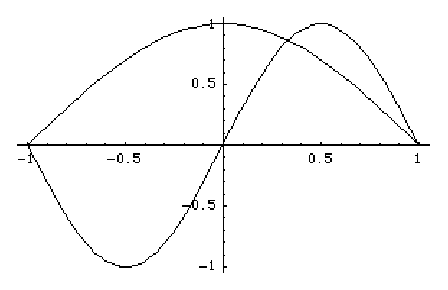
\includegraphics[scale=0.7]{wavefun1}
\end{figure}

The most probable values for position can be obtained from the squared wavefunctions:

\begin{figure}[htp!]
\centering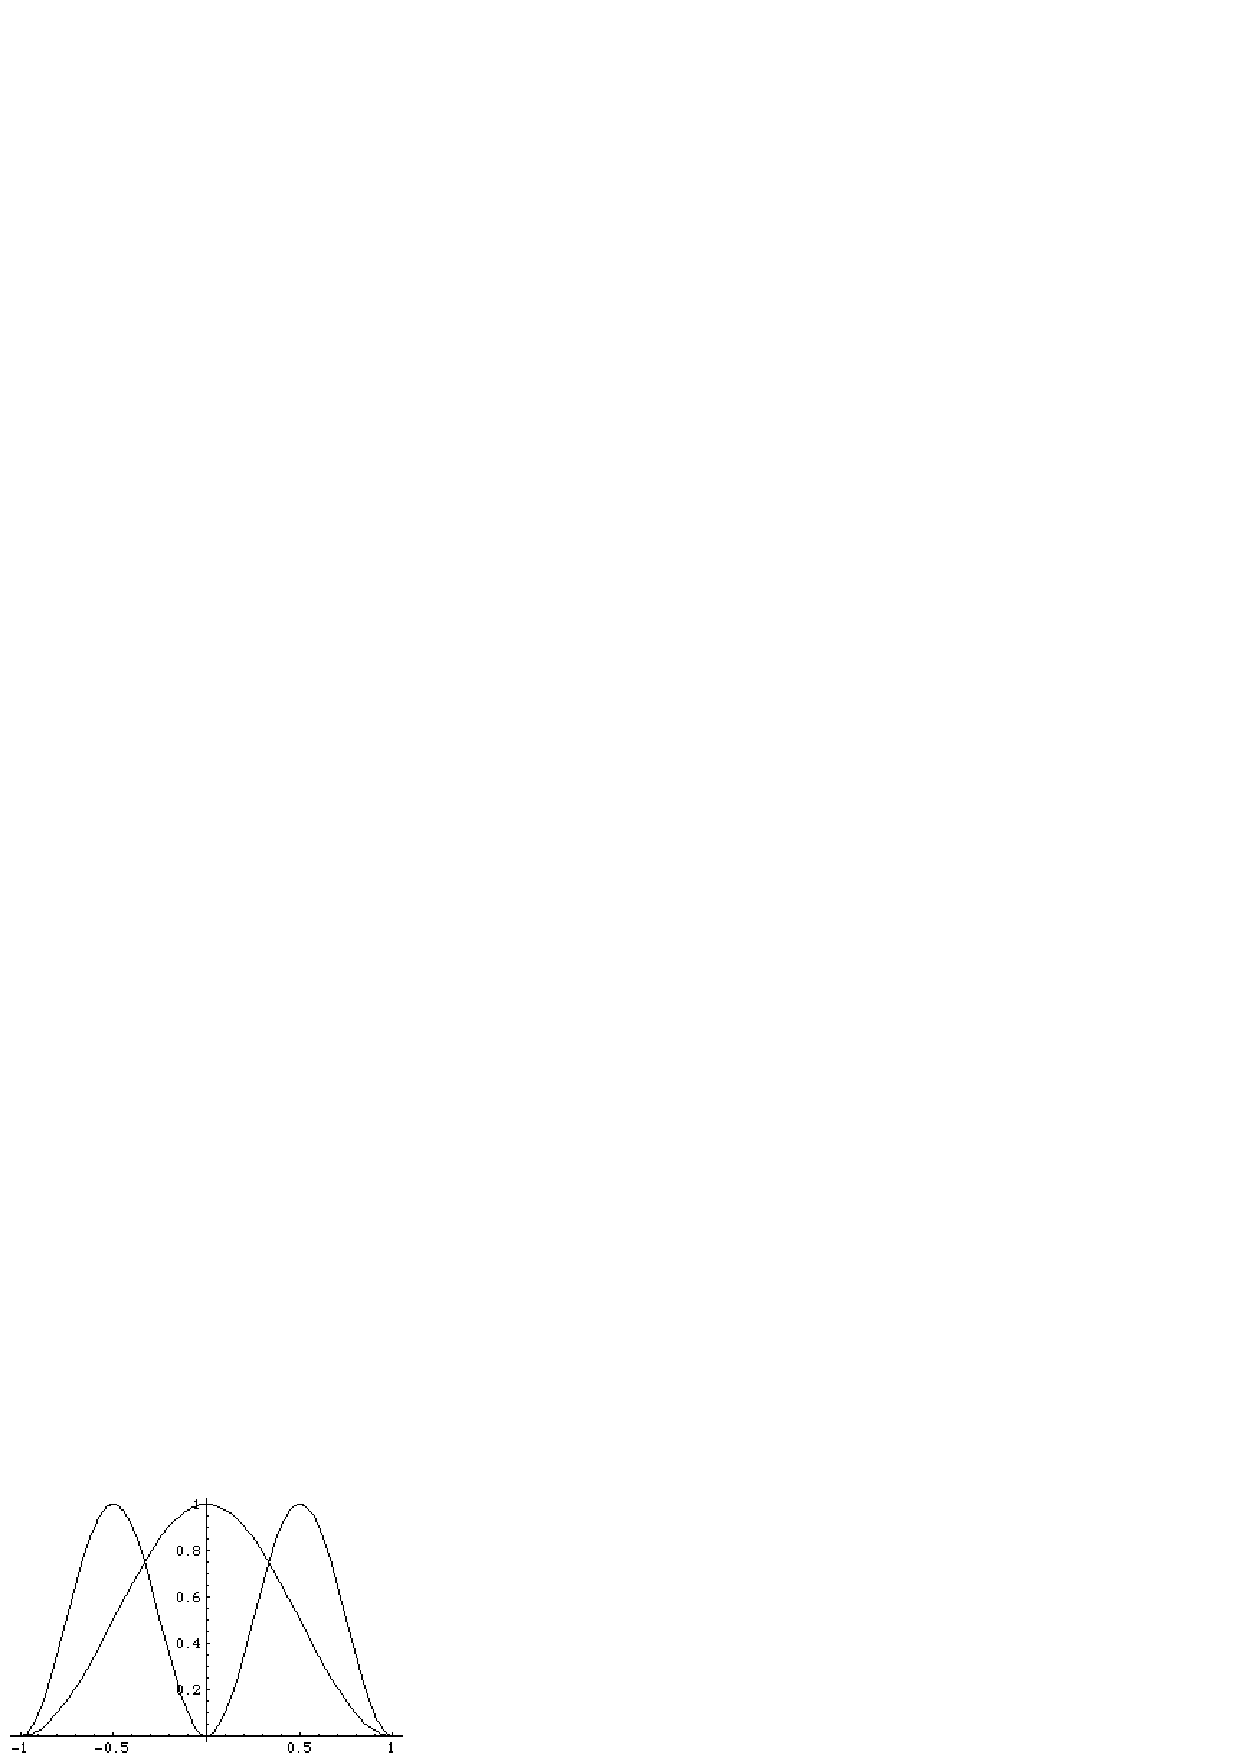
\includegraphics[scale=0.7]{wavefun2}
\end{figure}

$\psi_1$ has the maximum value at $r = 0$ whereas $\psi_2$ has two maxima at $\pm 0.5$. Note that on average both will give an outcome of $\left<\hat{r}\right> = 0$.

\item The most probable positions are given by the square of the wavefunction $\psi_0(x) = \left(2/L\right)^{1/2}\sin(3\pi x/L)$. The probability function is then $\left|\psi_0(x)\right|^2 \propto \sin^2(3\pi x/L)$. The extremum points for this function can be obtained by:
\begin{eqnarray}
\nonumber
& & \frac{d}{dx}\left(\sin^2(3\pi x/L)\right) = 0 \Rightarrow \sin(3\pi x/L)\cos(3\pi x/L) = 0\\
\nonumber
& & \Rightarrow \frac{3\pi x}{L} = n\pi\textnormal{ or }\frac{3\pi x}{L} = \left(n + \frac{1}{2}\right)\pi\\
\nonumber
& & \Rightarrow x = \frac{n}{3}L\textnormal{ or }x = \frac{n + 1/2}{3}L
\end{eqnarray}

Second derivatives can be used to identify the extrema:

$$\frac{d^2}{dx^2}\left(\sin^2(3\pi x/L)\right) \propto \cos^2\left(\frac{3\pi x}{L}\right) - \sin^2\left(\frac{3\pi x}{L}\right)$$

At $x = \frac{n}{3}L$ the values are positive which means that these correspond to (local) minima. For $x = \frac{n+1/2}{3}L$ the values are negative
and these points correspond to (local) maxima. For example, when $L = 2$ the probability function looks like:

\begin{figure}[htp!]
\centering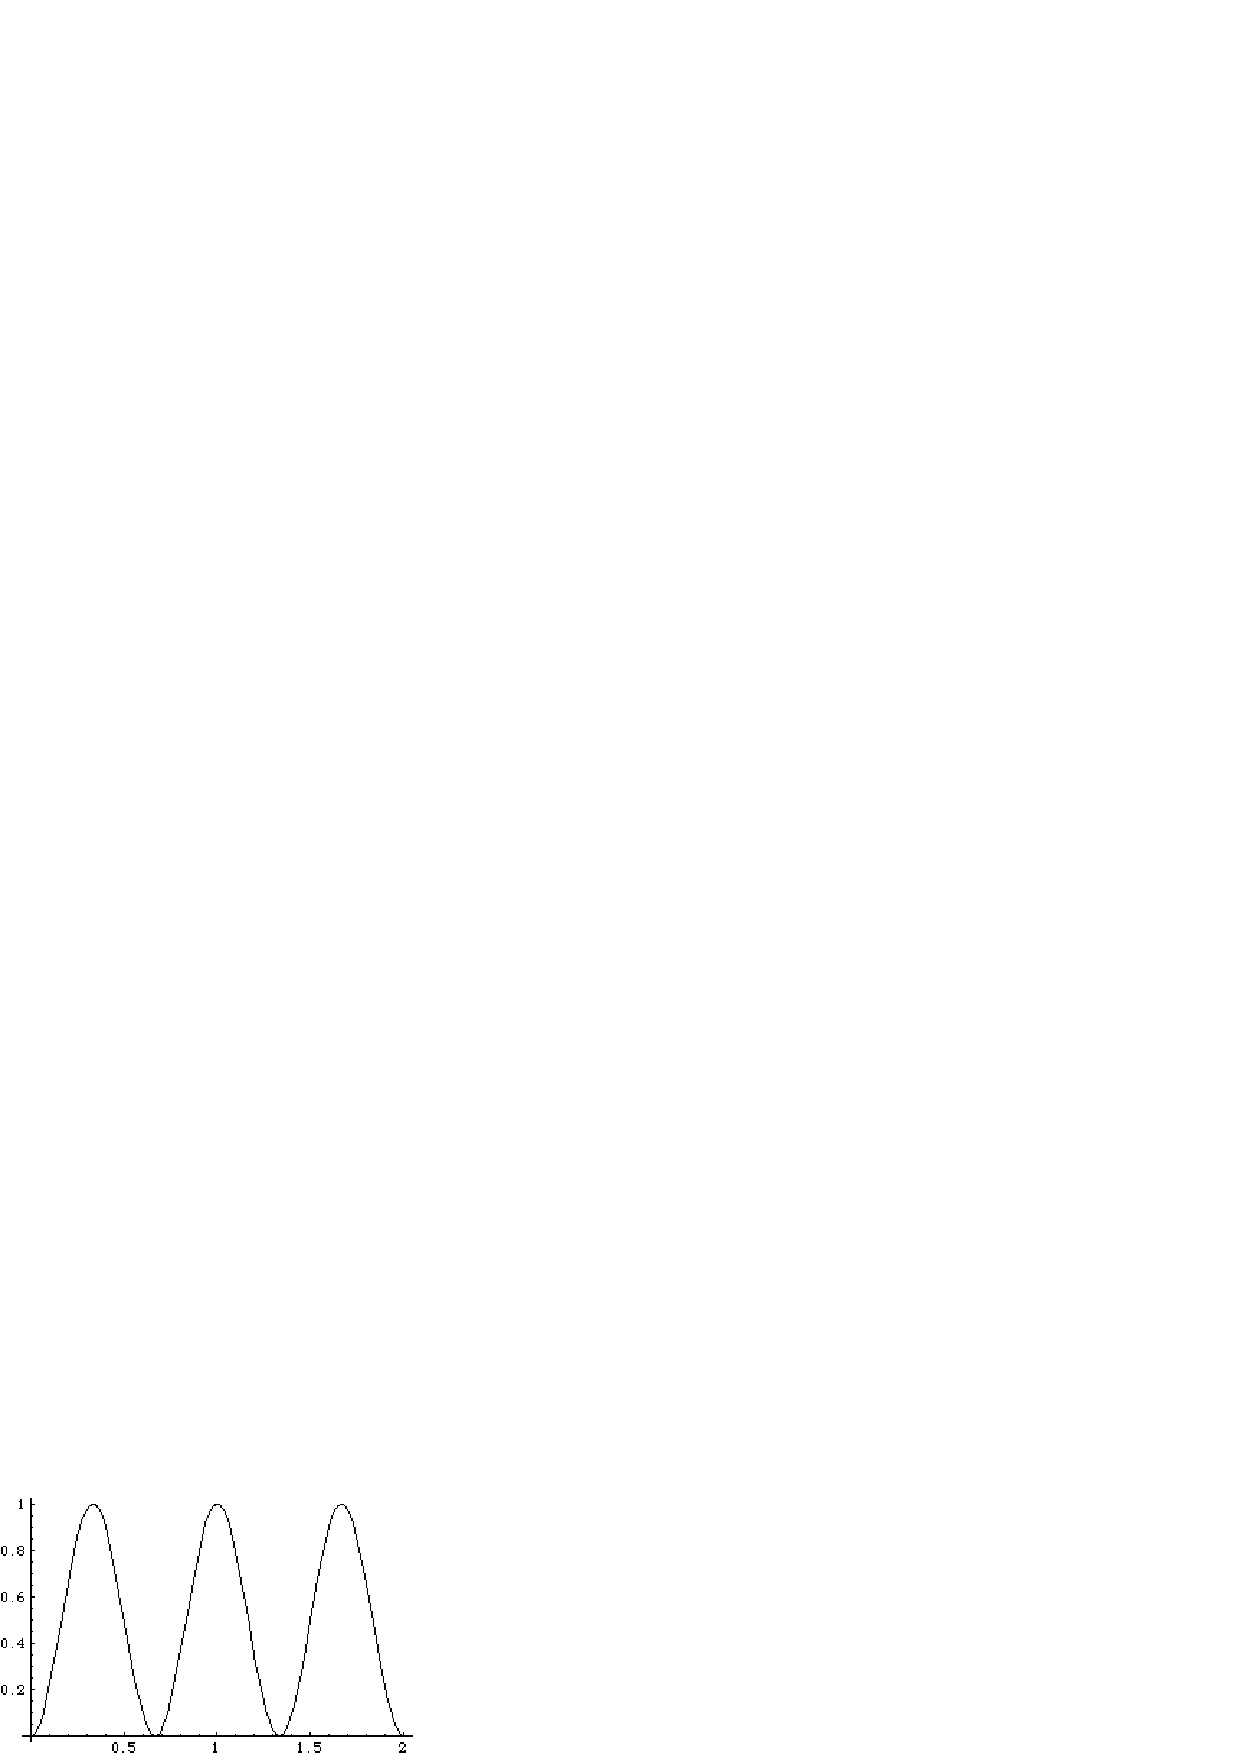
\includegraphics[scale=0.7]{wavefun3}
\end{figure}

\end{enumerate}

\hrule\vspace{0.5cm}
}{}

\item Derive the expressions for $V_c$ , $T_c$ and $P_c$ in terms of the van der Waals constants $a$ and $b$.

\ifthenelse{\equal{\solutions}{true}}{% Problem 6/1 solution
\noindent
\underline{Solution:}\\

The equations in the lecture notes can be rewritten as (the definition of critical point and the equation of state):

$$\frac{RT_c}{\left(\bar{V}_c - b\right)^2} = \frac{2a}{\bar{V}_c^3}$$
$$\frac{2RT_c}{\left(\bar{V}_c - b\right)^3} = \frac{6a}{\bar{V}_c^4}$$
$$P_c = \frac{RT_c}{\bar{V}_c - b} - \frac{a}{\bar{V}_c^2}$$

Division of the first equation by the second (side by side) yields $\bar{V}_c = 3b$. Substitution of this expression into the first equation above gives $T_c = \frac{8a}{27Rb}$. Substitution of the two previous equations into the last equation above yields $P_c = 
\frac{a}{27b^2}$. Note that the van der Waals constants $a$ and $b$ are usually calculated using the critical temperature and pressure since they are typically known more accurately than the critical volume.

\hrule\vspace{0.5cm}
}{}

\item The isothermal compressibility $\kappa$ of a gas is defined as:

$$\kappa = -\frac{1}{V}\left(\frac{\partial V}{\partial P}\right)_T$$

Calculate $\kappa$ for a van der Waals gas using the method of implicit differentiation (with respect to $P$). Show that in the limit of infinite volume, it yields $1/P$ (the same result as the ideal gas law).

\ifthenelse{\equal{\solutions}{true}}{% Problem 7/1 solution
\noindent
\underline{Solution:}\\

The current is proportional to the square the wavefunction ($\left|\psi(x)\right|^2$):
\begin{eqnarray}
\nonumber
& & I\propto \left|\psi(x)\right|^2 = B^2e^{-2Kx}\\
\nonumber
& & \frac{I_1}{I_2} = e^{-2K(x_1 - x_2)}\\
\nonumber
& & K=\left(2m_e\underbrace{(V - E)}_{=2\textnormal{ eV}}/\hbar^2\right)^{1/2}\\
\nonumber
& & = \left(\frac{2(9.11\times 10^{-31}\textnormal{ kg})(2.0\textnormal{ eV})(1.602\times 10^{-19}\textnormal{J/eV})}{(1.0546\times 10^{-34}\textnormal{ Js})^2}\right)^{1/2}\\
\nonumber
& & -2K(x_1 - x_2) = -2K\times(0.10\times 10^{-9}\textnormal{ m}) \approx 1.45\\
\nonumber
& & \Rightarrow \frac{I_1}{I_2} \approx 4.3
\end{eqnarray}

\hrule\vspace{0.5cm}
}{}

\item The cubic expansion coefficient is defined by

$$\alpha = \frac{1}{V}\left(\frac{\partial V}{\partial T}\right)_P$$

Calculate the cubic expansion and isothermal compressibility coefficients for an ideal gas.

\ifthenelse{\equal{\solutions}{true}}{% Problem 8/1 solution
\noindent
\underline{Solution:}\\
\begin{eqnarray}
\nonumber
& & \hat{H}\psi(r,\theta,\phi) = E\psi(r,\theta,\phi)\textnormal{ where }\hat{H}=-\frac{\hbar^2}{2I}\Lambda^2\\
\nonumber
& & \Lambda^2 = \frac{1}{\sin^2(\theta)}\frac{\partial^2}{\partial\phi^2} + \frac{1}{\sin(\theta)}\frac{\partial}{\partial\theta}\sin(\theta)\frac{\partial}{\partial\theta}
\end{eqnarray}

Since $-\frac{\hbar^2}{2I}$ is constant, it is sufficient to show that spherical harmonics are eigenfunctions of $\Lambda^2$. We operate on the given spherical harmonics by $\Lambda^2$.
\begin{enumerate}
\item $\Lambda^2Y_0^0(\theta,\phi) = \Lambda^2\frac{1}{2\sqrt{\pi}} = 0\textnormal{ (no angular dependency)}$. The rotation energy is $E = -\frac{\hbar^2}{2I}\times 0 = 0$. Also $L^2 = 0\times\hbar^2 \Rightarrow L = 0$ (since $\hat{L}^2 = -\hbar^2\Lambda^2$).
\item $\Lambda^2Y_2^{-1}(\theta,\phi) = \textnormal{ ...differentiation...} = -6Y_2^{-1}(\theta,\phi)$. The rotation energy is $E = -\frac{\hbar^2}{2I}\times (-6) = \frac{3\hbar^2}{I}$. Also $L^2 = 6\times\hbar^2 \Rightarrow L = \sqrt{6}\hbar$.
\item Expression for $Y_3^3$ was not given in the lecture notes. We use Maxima to obtain the expression: $Y_3^3(\theta,\phi) = \frac{5\sqrt{7}e^{3\phi i}\sin^3(\theta)}{8\sqrt{5\pi}}$. Then we need to evaluate: $\Lambda^2Y_3^3(\theta,\phi) = \textnormal{ ...differentiation...} = -12Y_3^3(\theta,\phi)$.
From this we can get the rotational energy as $E = \frac{6\hbar^2}{I}$. Also $L^2 = 12\times\hbar^2 \Rightarrow L = \sqrt{12}\hbar$.
\end{enumerate}

\hrule\vspace{0.5cm}
}{}

\item A certain gas has the following equation of state:

$$P = \frac{nRT}{V - nb}$$

\begin{itemize}

\item[a)] Calculate the following partial derivatives:

$$\left(\frac{\partial P}{\partial V}\right)_T\textnormal{ and }\left(\frac{\partial P}{\partial T}\right)_V$$

\item[b)] Show that the following relation holds for the mixed partial derivatives for this equation of state:

$$\left(\frac{\partial^2 P}{\partial V\partial T}\right) = \left(\frac{\partial^2 P}{\partial T\partial V}\right)$$

\end{itemize}

\ifthenelse{\equal{\solutions}{true}}{% Problem 9/1 solution
\noindent
\underline{Solution:}\\

The Hamiltonian for 2-D rotation is $\hat{H} = \frac{\hat{L}_z^2}{2I} = -\frac{\hbar^2}{2I}\frac{d^2}{d\phi^2}$ where the rotation axis is denoted by $z$ and $\phi$ is the angle of rotation.

\begin{enumerate}
\item Operate first by $\hat{L}_z$ on $e^{i\phi}$: $\hat{L}_ze^{i\phi} = -i\hbar\frac{d}{d\phi}e^{i\phi} = \hbar e^{i\phi}$. Thus $\hat{H}e^{i\phi} = \frac{\hbar^2}{2I}e^{i\phi}$.
\item The same reasoning gives: $\hat{L}_z e^{-2i\phi} = -i\hbar\frac{d}{d\phi}e^{-2i\phi} = -2\hbar e^{-2i\phi}$ and $\hat{H}e^{-2i\phi} = \frac{4\hbar^2}{2I}e^{-2i\phi}$.
\item The given wavefunction is not an eigenfunction of $\hat{L}_z$: $\hat{L}_z\cos(\phi) = -i\hbar\left(-\sin(\phi)\right)$ (expectation value is zero).
However, it is an eigenfunction of $\hat{H}$: $\hat{H}\cos(\phi) = -\frac{\hbar^2}{2I}\frac{d^2}{d\phi^2}\cos(\phi) = \frac{\hbar^2}{2I}\cos(\phi)$.
\item Operation by $\hat{L}_z$ would change the plus sign in the middle of the wavefunction into a minus, hence this is not an eigenfunction of $\hat{L}_z$. It is an eigenfunction of $\hat{H}$: $\hat{H}(\cos(\chi)e^{i\phi} + \sin(\chi)e^{-i\phi}) = -\frac{\hbar^2}{2I}\left((i)^2\cos(\chi)e^{i\phi} + (-i)^2\sin(\chi)e^{-i\phi}\right) = \frac{\hbar^2}{2I}\left(\cos(\chi)e^{i\phi} + \sin(\chi)e^{-i\phi}\right)$.
\end{enumerate}

\hrule\vspace{0.5cm}
}{}

\item Calculate the compressibility factor $Z$ for NH$_3(g)$ at 400 K and 50 bar by using the attached graph and the virial equation.

\begin{figure}[htp!]
\centering
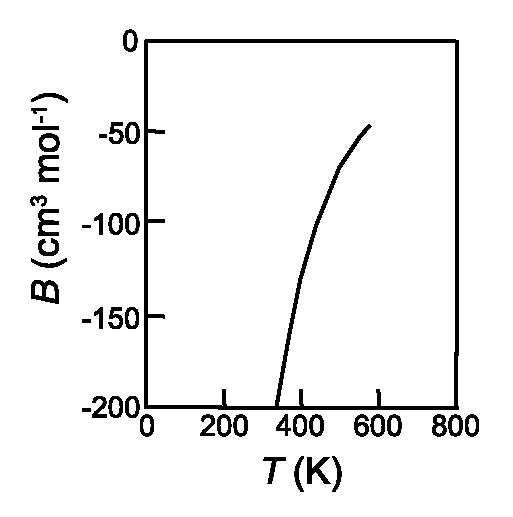
\includegraphics[scale=1.5]{graph}
\end{figure}

\ifthenelse{\equal{\solutions}{true}}{% Problem 10/1 solution
\noindent
\underline{Solution:}\\

By reading the value for $B$ from the graph, using relation $B' = B / RT$, and the virial equation written in terms of $P$, we get:

$$Z = 1 + B'P + ... = 1 + \frac{B}{RT}P + ...$$ 
$$\approx 1 + \frac{(-100\times 10^{-3}\textnormal{ L mol}^{-1})}{(0.0831451\textnormal{ bar L K}^{-1}\textnormal{ mol}^{-1})(400\textnormal{ K})}\times\left(50\textnormal{ bar}\right) = 0.85$$


\hrule\vspace{0.5cm}
}{}

\end{enumerate}
